\documentclass{article}       % onecolumn (second format)
\usepackage[utf8]{inputenc}
\usepackage[english]{babel}
\usepackage[document]{ragged2e}
\usepackage{graphicx}
\usepackage{amsmath,amssymb,amsthm} 
\usepackage{url}
\usepackage{xspace}
\usepackage[left=20mm,top=20mm]{geometry}
\usepackage{subcaption}
\usepackage{mathpazo}
\usepackage{booktabs}
\usepackage{hyperref}
\usepackage{tikz}
\usepackage{dsfont}
\usepackage[]{algorithm2e}
\usepackage[
  style=numeric,
  natbib=true,
  sortcites=true,
  block=space]{biblatex}
\bibliography{parts/biblio}
\newcommand\institute[1]{\newcommand\theinstitute{#1}}

\begin{document}

% The correct dates will be entered by the editor
\title{Integrating lexical constraints and background knowledge to $K$-Means with Deep Learning}
\author{Grand Maxence\\                                                   
        Supervised by : \\Gaussier \'Eric \and Thonet Thibaut \\ \and Tommasi Marc \and Bellet Aur\'elien  \and Moradi Fard Maziar } 
\date{\today}

\maketitle
%\twocolumn
\begin{abstract}
  We study in this paper the problem of thematic clustering with background
  knowledge. To perform K-Means with these constraints we need a representation
  where informations about documents and constraints are present. For this
  reason, deep $K$-Mean can be use to learn a latent space  showing all
  constraints, and perform $K$-Means in the latent space.
\end{abstract}

\section{Introduction}\label{sec:intro}

Clustering is one of the most fundamental tasks in data mining and machine
learning. $K$-Means algorithm is a clustering method using centroid models,
it represents each cluster by a single mean vector. $K$-Means clustering sorts
n objects into k clusters in which each observation belongs to
the cluster with the nearest centroid. This problem is computationally
difficult (NP-hard).
\begin{algorithm}
  \SetKwInOut{Input}{input}
  \SetKwInOut{Output}{output}
  \Input{Corpus C, the number of cluster K}
  \Output{Assignment matrix S}
  Let $r_1^{0}, r_2^{0} , ..., r_k^{0}$ be the initial centroids\\
  $t \gets 1$\\
  \Repeat{Convergence}{
    \For{i = 1 : N}{
      $
        S_{i,j}^t \gets \left\{
        \begin{array}{ll}
          1 & \mbox{if } j = \argmin_{k = \{1 ... K\}}||g(X_i) -
          r_k^{t-1}||_2^2\\
          0 & \mbox{Otherwise.}
        \end{array}
        \right.
      $
    }
    \ForEach{centroids $r_k$}{
      $r_k^t \gets \frac{1}{\sum_{i = 1}^N S_{i,k}}\sum_{i = 1}^N
      {X_i}S_{i,k}$.\\
    }
    $t++$\\
  }
  \Return{S}
  \caption{$K$-means}
\end{algorithm}
\\Given a corpus C, where each document X is a 
d-dimensional real vector, k-means clustering aims to partition the n 
documents into K clusters represented by centroids 
R = {$r_1, r_2, ..., r_K$}. S is the assignment matrix :
\begin{equation*}
  S_{i,j} = \left\{
\begin{array}{ll}
  1 & \mbox{if document i $\in$ cluster j}\\
  0 & \mbox{Otherwise.}
\end{array}
\right.
\end{equation*}
Formally, the objective is to minimize :
$$
\sum_{i =1 }^N ||X_i - RS_i ||_2^2
$$
In real application domains, users may want to introduce constraints to finding 
useful properties for clustering data. The difficulty with integration of 
constraints into $K$-Means algorithm is to find a good representation for data 
taking into account constraints. The Deep Learning and Auto-Encoder can be used 
to learn this representation. With Auto-Encoder we have to perform the $K$-Means 
in the latent space learned.
\\The major contribution to this work, is to propose a constrained Deep $K$-Means 
taking account into ML and CL constraints and lexical constraints.
\\In the next section, we provide some background on the $K$-Means algorithm and 
deep learning. In section 3, we proposed a method to introduce constraints to 
the $K$-Means algorithm. And we are experimenting our method in section 4.

\section{Background}\label{sec:related}
\subsection{$K$-Means}
Given a corpus C, where each document X is a 
d-dimensional real vector, k-means clustering aims to partition the n 
documents into K $S_k$ clusters represented by centroids 
R = {$r_1, r_2, ..., r_K$}.
Formally, the objective is to minimize :
$$
\sum\limits_{k =1 }^K \sum\limits_{X \in S_k} ||X - r_k||_2^2
$$
We can see $K$-Means in algorithm\ref{algo:kmeans}
\begin{algorithm}
  \SetKwInOut{Input}{input}
  \SetKwInOut{Output}{output}
  \Input{Corpus C, the number of cluster K}
  \Output{Assignment matrix S}
  Let $r_1^{0}, r_2^{0} , ..., r_k^{0}$ be the initial centroids\\
  $t \gets 1$\\
  \Repeat{Convergence}{
    \ForAll{$X \in C$}{
      $
        S_{k}^t \gets \{ X : ||X - r_k^{t-1}||_2^2 \leq ||X - r_l^{t-1}||_2^2 \forall l \neq k, 1 \leq l \leq K \}
      $\\
    }
    \ForEach{centroids $r_k$}{
      $r_k^t \gets \frac{1}{|S_k^t|}\sum\limits_{X \in S_k^t}X$.\\
    }
    $t \gets t+1$\\
  }
  \Return{S}
  \caption{\label{algo:kmeans}$K$-means}
\end{algorithm}

\subsection{Auto-Encoder}
The Auto-Encoder~\cite{Goodfellow-et-al-2016} allows to learn a latent space with significant
information for the clustering without loss of information.
The Auto-Encoder tries to learn a function $f (X, \theta) = X$. In
other words, it is trying to learn an approximation of the identity
function. An Auto-Encoder is composed in two parts an encoder function
g, and a decoder function f. To learn representations from which it is 
possible to reconstruct input data,, we use a
reconstruct loss $L_{rec}$ using MSE :
\begin{equation}
  L_{rec}(X, \theta) = || X - A(X, \theta) ||_2^2 
\end{equation}
where $A(X, \theta) = f(g(X, \theta))$ is the Auto-Encoder output. We denote 
$h_\theta(X) = g(X,\theta)$ the encoder output.
\begin{figure}[!h]
  \centering
  \resizebox{\hsize}{!}{
    \fbox{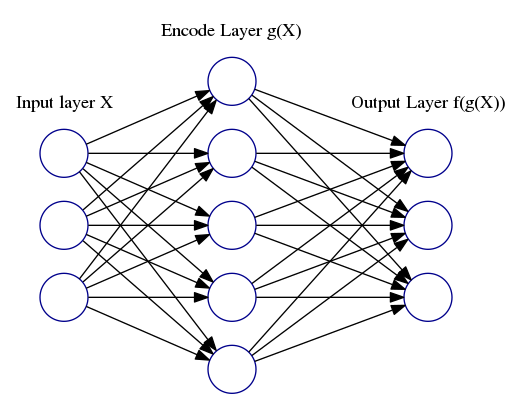
\includegraphics{parts/res/autoencoder.png}}
  } 
  \caption{Auto-Encoder}
  \label{fig:autoenc}
\end{figure} 
\subsection{\label{seq:DeepClust}Deep Clustering}
A several approaches for the deep $K$-Means propose to jointly learn the
representation and perform the $K$-Means algorithm \cite{2018arXiv180107648A}.
In these approaches, network's loss is divided in two parts :
The non-clustering loss does not
take into account of the clustering parts. In general, the non-clustering 
loss is the reconstruction loss of the auto-encoder. We can add additional 
information in the non-clustering loss to bias the representation. For
example, in our case, we add penalties to integrate lexical constraints
.
The clustering loss allows to learn a  $K$-means friendly representation.
Moradi Fard, Thonet and Gaussier \cite{Deap-K-Means} proposed a method for deep $K$-Means 
clustering based on a continuous reparametrization of the objective function 
that leads to a truly joint solution. 
The problem takes the form : 
\begin{equation}
L(C ,\alpha;\theta,R) = \sum\limits_{X \in C} ||X - A(X;\theta)||_2^2 + 
\lambda_0 \sum\limits_{X \in C}||h_\theta(X) - c(h_\theta(X); R) ||_2^2
\end{equation}
where $c(g(X; \theta); R) = \argmin\limits_{k = 1 .. K} || h_\theta(X) - r_k||_2^2$
is a non differentiable function that assigns the document X
to its nearest centroid.\\
They transform this representation as follows :
\begin{equation}
L(C ,\alpha;\theta,R) = \sum\limits_{X \in C} ||X - A(h_\theta(X))||_2^2 + 
\lambda_0 \sum\limits_{X \in C}\sum\limits_{k=1}^K||h_\theta(X) - r_k ||_2^2 G_{k}(h_\theta(X), \alpha; R) 
\end{equation}
where $G_{k}$ is a differentiable function such that :
\begin{equation}
  \lim\limits_{\alpha \rightarrow \alpha_0}G_{k}(h_\theta(X), \alpha; R) = \left\{
\begin{array}{ll}
  1 & \mbox{if} r_k = c(h_\theta(X); R)\\
  0 & \mbox{Otherwise.}
\end{array}
\right.
\end{equation}
where $\alpha$ play the role of an inverse temperature. In \cite{Deap-K-Means}
, $G_{k}$ was chosen to be a parameterized softmax : 
$G_{k}(h_\theta(X), \alpha; R) = \frac{e^{-\alpha F(h_\theta(X),r_k)}}
{\sum\limits_{k' = 1}^K e^{-\alpha F(h_\theta(X),r_k')}}$\\
To update $(\theta, R)$, they used the stochastic gradient descent (SGD)
as follows :
\begin{equation}
  (\theta, R) \gets (\theta, R) - \epsilon \frac{1}{|\widetilde{C}|}
  \nabla_{(\theta, R)} L(C, \alpha; \theta, R)
\end{equation}
where $\widetilde{C}$ is a random mini batch of C, and $\epsilon$ the
learning rate.
Algorithm \ref{algo:dkm} summarizes the deep k-Means algorithm :
\begin{algorithm}[!h]
  \SetKwInOut{Input}{input}
  \SetKwInOut{Output}{output}
  \Input{Corpus C , number of clusters K, balancing parameter $\lambda_0$,
    scheme for $\alpha$, number of epochs T ,
    number of minibatches MB , learning rate $\epsilon$}
  \Output{Auto-Encoder parameter $\theta$, cluster representative R}
  Initialize $\theta$ and $r_k$, $1 \leq k \leq K$ (randomly or through 
  pretraining)\\
  \ForEach{$\alpha = m_\alpha : M_\alpha$}{
    \ForEach{t = 1 : T}{
      \ForEach{n = 1 : MB}{
        Draw minibatch $\widetilde{C} \subseteq  C$\\
        Update ($\theta, R$) using SGD
      } 
    }  
  }
  \caption{\label{algo:dkm}Deep $K$-Means}
\end{algorithm}

\section{Proposed Method}
The idea is to learn a latent space taking into account lexical constraints and
background knowledge.
\\We denote $KW = \begin{pmatrix} kw_1 & kw_2 & ... & kw_{k-1} & kw_{k}
\end {pmatrix}$
the set of index of keywords. X a document of size n,
X' the vector showing only informations about keywords such that :
\begin{equation*}
\forall_{i=1,2,..,n}X_i' = \left\{
\begin{array}{ll}
  X_i & \mbox{if } i \in KW \\
  0 & \mbox{Otherwise.}
\end{array}
\right.
\end{equation*}
C the corpus, N the size of C, and K the number of cluster.
\subsection{Auto-Encoder}
We denote $h_X$ the encoder output : 
\begin{equation}\label{eq:h}
  h_X = g(X,\theta)
\end{equation}
\subsubsection{Lexical Constraints}
To learn the latent space we a use sparse penalty such that the representation
of the document X is close of the representation of X'. In this way, in the
latent space, the representation of document will be biased by keywords.
We introduce a sparse penalty $\omega_{KW}$ for lexical constraints and
use squared loss : 
\begin{equation}\label{eq:omega1}
  \omega_{KW} = \sum_{\forall{X\in C}} || h_X - g(X',\theta) ||_2^2 =
  \sum_{\forall{(X,X')\in X}} || h_X - h_{X'}||_2^2
\end{equation}
\subsubsection{Backgroung Knowledge}
In addition of lexical constraints we introduce background knowledge, so we need
a representation taking into account these constraints.\\
For must-link constraints we want close representations for each pair $X_1$, $X_2$
in the set ML. We introduce a sparse penalty $\omega_{ML}$ for must-link
constraints and use squared loss :
\begin{equation}\label{eq:omegaML}
  \omega_{ML} = \sum_{\forall{(X_1,X_2)\in ML}} || h_{X_1} - h_{X_2} ||_2^2
\end{equation}
For cannot-link constraints we want distant representations for each pair $X_1$, $X_2$
in the set CL.
We can use the hinge loss.
We introduce a sparse penalty $\omega_{CL}$ for cannot-link constraints.
\begin{equation}\label{eq:omegaCL}
  \omega_{CL} = \sum_{\forall{(X_1,X_2)\in CL}} max(0,
  \eta - || h_{X_1} - h_{X_2} ||_2^2)
\end{equation}
The sparse penalty is :
\begin{equation}\label{eq:Sparse}
  \Omega(C) = \omega_{KW} + \omega_{CL} + \omega_{ML}  
\end{equation}

Then the reconstruct loss function is :
\begin{equation}\label{eq:AEDK}
  L_{rec}(C, \theta) = \sum_{X \in C}(||X - f(g(X, \theta))||_2^2
\end{equation}
Finally the loss function for the Auto-Encoder is :
\begin{equation}\label{eq:AE}
  L_{SAE}(C,KW; \theta) = L_{rec}(C, \theta) + \Omega(C)  
\end{equation}

\subsection{Deep K-Means}

\subsubsection{Clustering Loss}

For the clustering loss we can use squared loss with euclidian distance. We
denote $r = \begin{pmatrix} r_1 & r_2 & ... & r_K\end{pmatrix}$ the vector of
centroids.  
\begin{equation}\label{eq:loss_clust}
  L_{clust}(C,K) = \sum_{i=1}^K \sum_{X \in K_i} ||h_X - r_i ||_2^2 
\end{equation}
Finally the loss function is :
\begin{equation}\label{eq:loss_FINALE}
  Min~L(KW, C, K; \theta) = \epsilon_0.L_{SAE}(C, KW; \theta) 
  + \epsilon_1.L_{clust}(C,K)
\end{equation}

with $\epsilon_0 \geq 0$, $\epsilon_1 \geq 0$.

\section{Experiment}

\subsection{Data}
To experiment our algoritm we use two corpus $C_1$ and $C_2$. $C_1$ contains a
set of documents related to Finance and $C_2$ contains a set of documents
related to Sport Each coprus are divided in 10 classes.

\subsection{Evaluation}
\subsubsection{Reference Algorithm}
We evaluate our algorithm with three algorithms :
\begin{itemize}
\item \textbf{NNclustering} proposed by Hsu and Kira
\cite{2015arXiv151106321H}.
\item \textbf{COPKmeans} proposed by Wagstaff \cite{Wagstaff:2001:CKC:645530.655669}.
\item \textbf{Thematic kmeans}, the loss function for this algorithm is
  \begin{equation*}
    argmin \sum_{i=1}^{N}L(x_i) + \beta\sum_{k=1}^{K}||r_k - \sum_{\omega \in K}
    \alpha_{k,\omega}h(\omega, \theta)||_2^2 + \delta\sum_{k=1}^{K}||\alpha_k|| 
  \end{equation*}
  with $L(x_i) = L_{rec}(x_i) + \lambda L_{clust}(x_i)$
\end{itemize}
\subsubsection{Metric}
To evaluate our algorithm and compare results with reference algorithms we can
use the NMI metric and Purity Metric \cite{measure}. The NMI metric is defined by
$$
NMI(S,C) = \frac{I(S,C)}{[H(S)+H(C)]/2}
$$ 
with
$$
I(S,C) =\sum_k \sum_f\frac{|s_k \cap c_f|}{N}log\frac{N|s_k \cap c_f|}{|s_k| |c_f|}
$$
and 
$$
H(S) = -\sum_k\frac{|s_k|}{N}log\frac{N|s_k|}{|s_k|}
$$.
The purity metric is defined by :
$$
purity(S,C) = \frac{1}{N}\sum_k {max}_j|s_k \cap c_j|
$$
\subsection{Separate Corpus }
With corpus $C_1$ and $C_2$ we generate $KW_1$ the set of keywords
for $C_1$ and $KW_2$ the set of keywords for $C_2$. Then we denote $KW$
the set of keywords for clustering such that $KW = KW_1 \cup KW_2$.\\
To generate $KW_1$ (resp $KW_2$) we extract keywords from $C_1$ (resp $C_2$)
with RAKE algorithm \cite{rake}.\\
For must-link constraints we extract a set of pairs $(X_1, X_2)$ from each
corpus such that $(X_1, X_2) \in C_1 \vee (X_1, X_2) \in C_2$.
And for cannot-link constraints we extract a set of pairs $(X_1, X_2)$ from
each corpus such that $(X_1 \in C_1 \wedge  X_2 \in C_2)\vee (X_1 \in C_2 \wedge
X_2 \in C_1)$.\\
The purpose of the experiment is to rediscover the different corpus $C_1$ and
$C_2$ with keywords and background knowledge.
\subsection{Noising Text}
With corpus $C_1$ and $C_2$ we generate $KW$ the set of keywords
for $C_1$.
To generate $KW$ we extract keywords from $C_1$ with RAKE algorithm \cite{rake}.
For must-link constraints we extract a set of pairs $(X_1, X_2)$ from Corpus
$C_1$, with $X_1$, $X_2$ in the same class.
And for cannot-link constraints we extract a set of pairs $(X_1, X_2)$ from Corpus
$C_1$, with $X_1$, $X_2$ in different classes.
Then we concatenate documents from $C_1$ with documents from $C_2$.\\
The purpose of the experiment is to rediscover the different classes of the
corpus $C1$ with keywords and background knowledge.

%\section{Conclusion}

%\section{Future Works}
In future works, we plan to test pairwise constraints.
To test these  constraints, we need another baseline algorithm. For
lexical constraint we only used deep $K$-Means algorithm. We can use this
algorithm, but we have to also use algorithm taking into account pair. We can 
use COP$K$-Means algorithm like baseline.\\ 
To test the integration of pairwise constraints with lexical constraints we can 
use an alternative form of the  COP$K$-Means algorithm. We learn a $k$-means 
friendly space taking into account lexical constraints and perform COP$K$-Means
in the learned latent space. The loss function for this model is :
\begin{equation}
\begin{array}{l l}
  Min~L(KW, C, K; \theta) = &(L_{rec}(C, \theta) + \omega_{KW} )
\\ & + \lambda.L_{Clust}(X, K;R, \theta)
\end{array}
\end{equation}
Then, we can test the robustness of our model in different ways.
First we can change the number of extracted keywords by class, in
our tests, we extracted 3 keywords by class, but we can imagine, experiments 
where the number of keywords is higher or lower, or where the number of 
extracted keywords for each class is different. Then we can change the number
of clusters.
%\begin{acknowledgements}
Merci les gens
\end{acknowledgements}

\newpage
\nocite{*}
\printbibliography[title=References]

\end{document}
\grid
